\classheader{12-01-2017}

What is the fundamental group of the one-point union of two circles? (This is often called the `wedge' or `bouquet' of two circles.)

\begin{figure}[!htb]
	\centering
	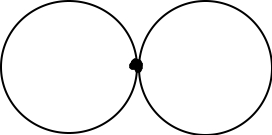
\includegraphics[scale=.5]{images/wedge2circ}
	\caption{The one-point union of two circles}
	\label{fig:wedge2circ}
\end{figure}


A covering space looks like a (connected) directed graph with labeled, oriented edges.

\begin{figure}[!htb]
	\centering
	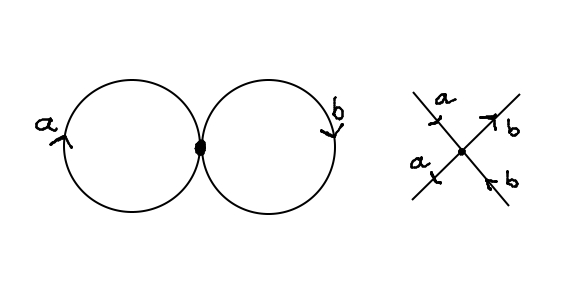
\includegraphics[scale=.5]{images/wedge2circcov}
	\caption{A covering space and the intersection schema for the wedge of two circles}
	\label{fig:wedge2circcov}
\end{figure}


\begin{figure}[!htb]
	\centering
	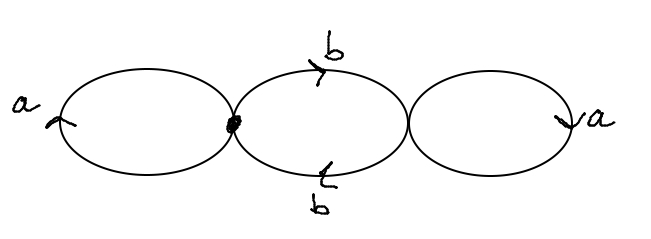
\includegraphics[scale=.5]{images/wedge2circcov2-1}
	\caption{A two-to-one cover of the wedge of two circles}
	\label{fig:wedge2circcov2-1}
\end{figure}



\begin{figure}[!htb]
	\centering
	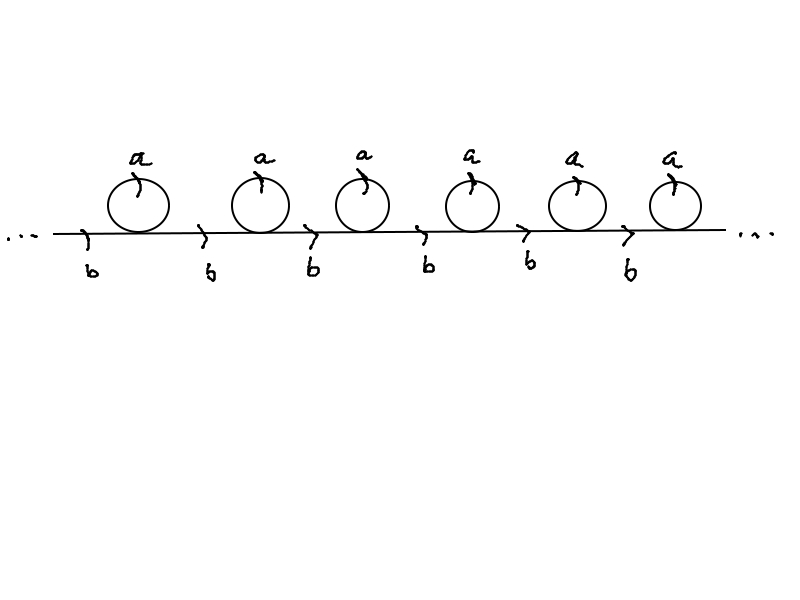
\includegraphics[scale=.5]{images/wedge2circcovinf}
	\caption{An infinite-sheet cover of the wedge of two circles}
	\label{fig:wedge2circcovinf}
\end{figure}

What is the fundamental group of this space? It turns out that it is the group $\langle a,b|\rangle$, the free group on two generators.

\begin{figure}[!htb]
	\centering
	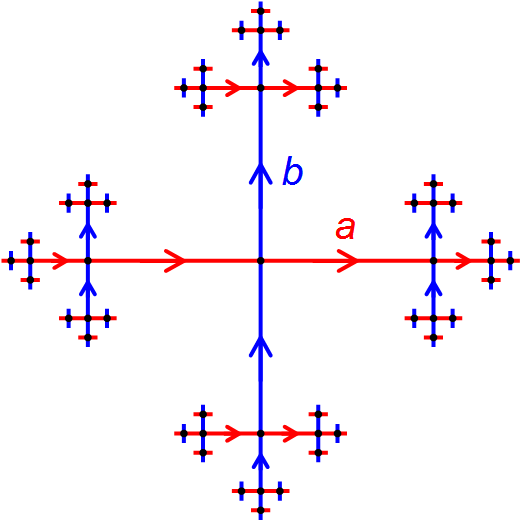
\includegraphics[scale=.5]{images/F2_Cayley_Graph}
	\caption{A cover with no loops}
	\label{fig:f2cayley}
\end{figure}

Looking at \ref{f2cayley}, we can see that a path in the wedge of two circles lifts to a path from some point $x_0$ to some point $x_1$ in this cover.  Such a path is unique, as there are no loops in the covering space.  Hence the only trivial words on the generators are of the form $ww^{-1}$, which defines the free group on two generators.

In general, the wedge of $k$ circles has the free group on $k$ generators as its fundamental group.

